\documentclass[aps, prl, longbibliography, linenumbers, superscriptaddress]{revtex4-2} 

\usepackage{graphicx,color}  % needed for figures
\usepackage{dcolumn}   % needed for some tables
\usepackage{bm}        % for math
\usepackage{textcomp}
\usepackage[section]{placeins}
\usepackage{ulem}
\usepackage{float}
\usepackage{epsfig,amssymb,amsmath,amsthm,amsfonts,amsbsy,mathrsfs}
\usepackage{eqnarray}
\usepackage{multirow}
\usepackage{array}
\usepackage{ifthen}
\usepackage[displaymath]{lineno}

%%%%%%%%%%%%%%%%%%%%%%%%%%%%%%%%%%%%%%%%%%%%%
\ifthenelse{1>0}{
	\newcommand{\blue}{\color{blue}}
	\newcommand{\red}{\color{red}}
	\newcommand{\green}{\color{green}}
	\newcommand{\magenta}{\color{magenta}}
}
{
	\newcommand{\blue}{}
	\newcommand{\red}{}
	\newcommand{\green}{}
	\newcommand{\magenta}{}
}

%%%%%%%%%%%%%%%%%%%%%%%%%%%%%%%%%%%%%%%%%%%%
%change equation label
\makeatletter
\usepackage{subfigure}
\setcounter{equation}{0}
\setcounter{figure}{0}
\renewcommand\theequation{S\arabic{equation}}
\renewcommand\thefigure{S\arabic{figure}}

%%%%%%%%%%%%%%%%%%%%%%%%%%%%%%%%%%%%%%%%%%%%
%fix revtex4-2
\makeatletter
\let\newfloat\newfloat@ltx
\makeatother

%%%%%%%%%%%%%%%%%%%%%%%%%%%%%%%%%%%%%%%%%%%%
%cref equations
\usepackage[capitalise]{cleveref}

%%%%%%%%%%%%%%%%%%%%%%%%%%%%%%%%%%%%%%%%%%%%
% pesudo code
\usepackage{algorithm}
\usepackage{algorithmic}
\renewcommand{\algorithmicrequire}{\textbf{Input:}}
\renewcommand{\algorithmicensure}{\textbf{Output:}}
%%%%%%%%%%%%%%%%%%%%%%%%%%%%%%%%%%%%%%%%%%%%
\newcommand{\dif}{\mathop{}\!\mathrm{d}}
\newcommand{\I}{\mathrm{i}}
\newcommand{\grad}{\nabla}
\newcommand{\dive}{\nabla \cdot}
\newcommand{\del}{\nabla^2}
\newcommand{\order}{\ensuremath{ \mathcal{O} }}
\newcommand{\pd}[2]{\frac{\partial{#1}}{\partial{#2}}}
\newcommand{\pdd}[2]{\frac{\partial^2{#1}}{\partial{#2}^2}}
\newcommand{\ts}{\textsuperscript}
\newcommand{\code}[1]{\texttt{#1}}
\newcommand{\TODO}{\colorbox{blue}{ \begin{minipage}{0.06\textwidth} \centering \color{magenta} TODO \end{minipage} } }
\NewDocumentCommand{\codeword}{v}{ \texttt{#1} }

%%%%%%%%%%%%%%%%%%%%%%%%%%%%%%%%%%%%%%%%%%%%

\begin{document}
\title{Supplemental Material}

\author{Jialiang Wei}
\affiliation{School of Physics, Peking University, Beijing, China}
\author{Yichen Yan}
\affiliation{Center for Quantitative Biology, Peking University, Beijing, China}
\affiliation{Peking-Tsinghua Center for Life Sciences, Peking University, Beijing, China}
\author{Jie Lin}
\email{linjie@pku.edu.cn}
\affiliation{Center for Quantitative Biology, Peking University, Beijing, China}
\affiliation{Peking-Tsinghua Center for Life Sciences, Peking University, Beijing, China}
\date{\today}

\maketitle
 
\subsection{I. Cell cycle-dependent growth rate}

\begin{figure}[htb!]
	\centering
	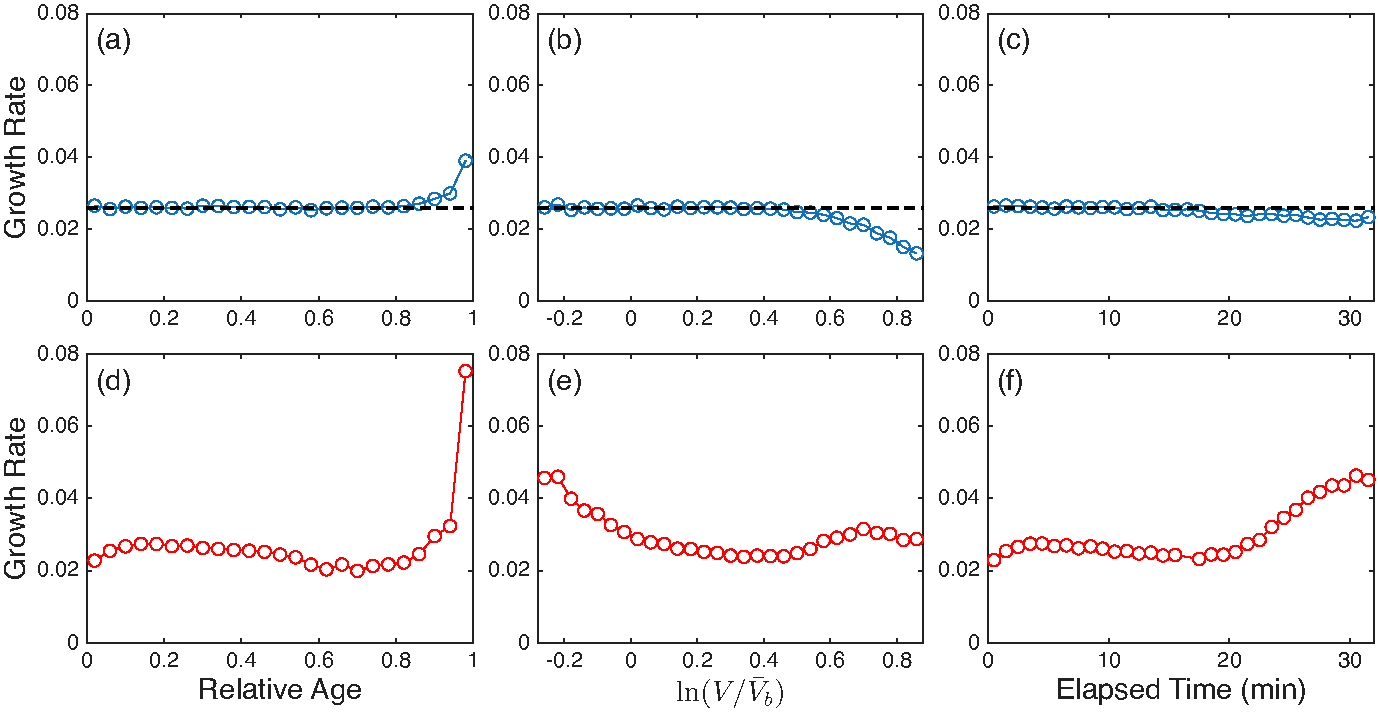
\includegraphics[width=1.0\textwidth]{average}
	\caption{Cell cycle-dependent average growth rate. (a-c) The growth rate $\lambda =\langle  \Delta x / \Delta t \rangle $ averaged over cell cycles for the simulation data vs. relative age (a), $x\equiv \ln(V/\bar V_b)$ (b), and the elapsed time (c). The black dashed line is the ground truth for the average growth rate. (d-f) The same analysis as (a-c) but for the experimental data as shown in Fig.~1(a) of the main text.}
	\label{fig:trajectory}
\end{figure}

\begin{figure}[htb!]
	\centering
	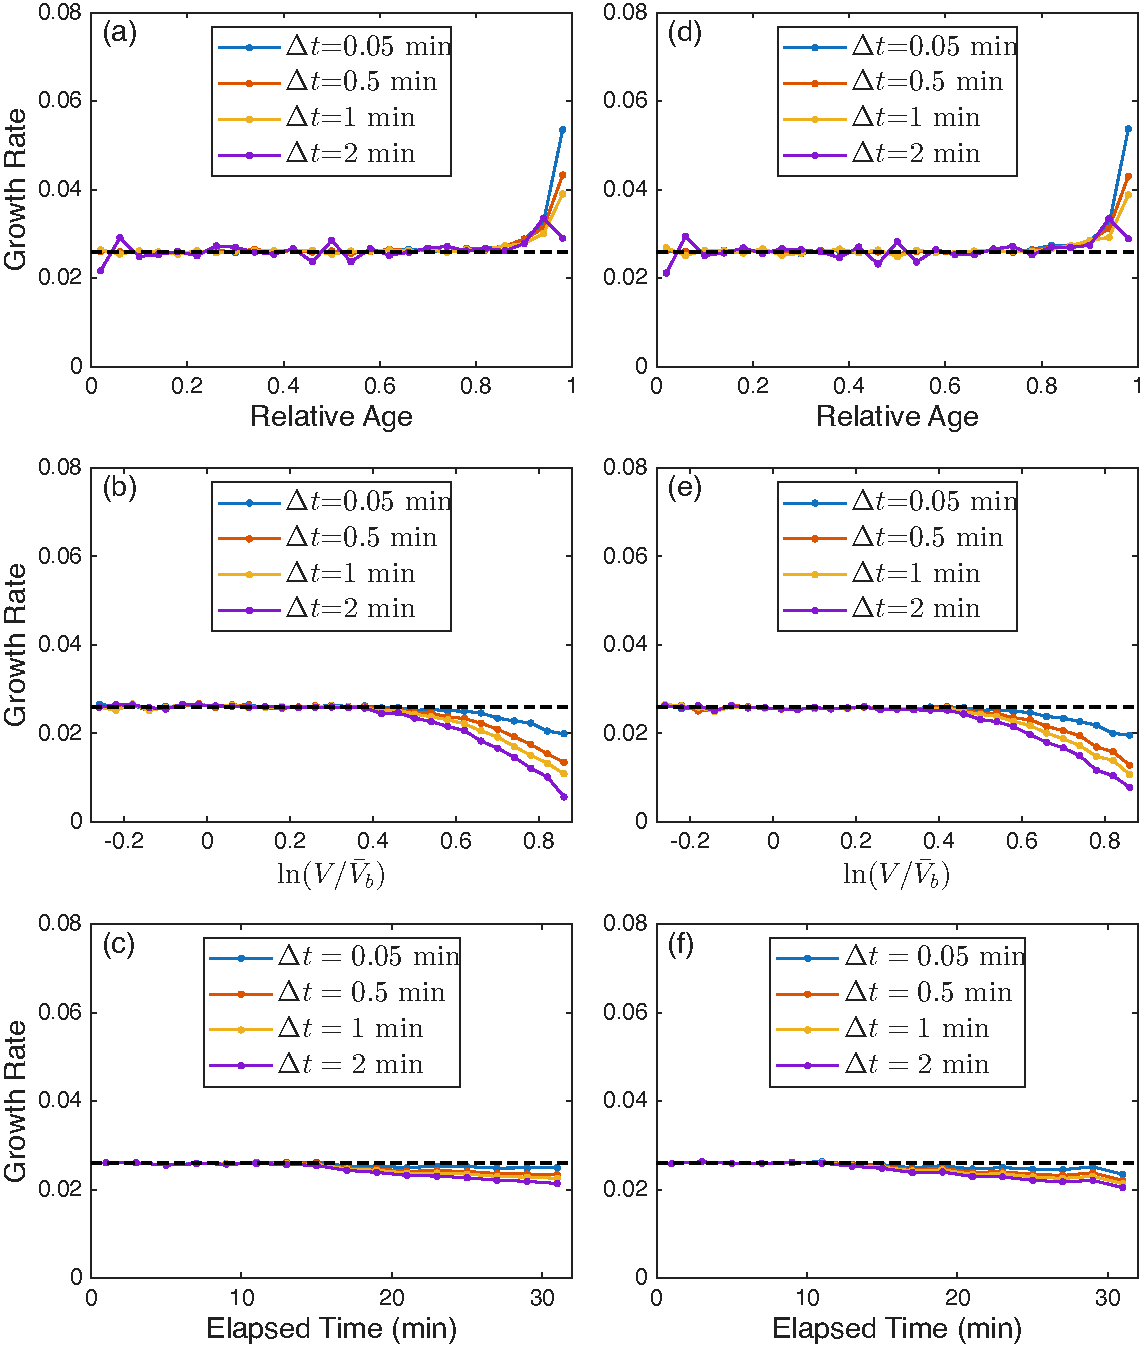
\includegraphics[width=0.8\textwidth]{deltat.pdf}
	\caption{Cell cycle-dependent growth rate for different time intervals and additional models. (a-c) The same analysis as Fig.~\ref{fig:trajectory}(a-c), but for different time intervals to compute the growth rate. For the relative-age statistics, the apparent growth acceleration near the cell-cycle end does not diminish as $\Delta t$ decreases. In contrast, for the relative-volume and elapsed-time statistics, the deviation from the ground-truth constant growth rate decreases with a smaller $\Delta t$, confirming that this reduction bias stems from the finite time interval. (d-f) The same analysis as (a-c), but the deterministic growth rate varies across cell cycles with a coefficient of variation (CV) of 0.1, roughly consistent with experimental measurements \cite{Taheri2015cell}. The statistical bias is robust against the randomness in the deterministic growth rate across cell cycles.}
	\label{fig:deltat}
\end{figure}

% {\blue Notably, the experimental data in (g) exhibit an apparent rapid initial growth at cell birth, a feature absent in the white-noise simulation (d) but later captured by the colored-noise model (Fig.~\ref{fig:colored}).} 8

%We introduce a minimal model of cell volume growth as a control for the experimental data and define $x\equiv \ln(V/\bar V_b)$ where $V$ is the cell volume and $\bar V_b$ is the birth volume averaged over cell cycles, which is a constant. In the minimal model, $x$ follows a drifted Brownian motion:
%\begin{equation}
%	\mathrm{d}x = a \mathrm{d}t + b \mathrm{d}W.
%	\label{eq:GBM}
%\end{equation}
%Here, $t$ is time, $a$ is the deterministic growth rate, and $b$ is the noise intensity. $\mathrm{d}W$ represents a Wiener process increment, which is a Gaussian-distributed random number with mean equal to zero and variance equal to $\mathrm{d}t$ \cite{Gardiner2004handbook}. Cell division is implemented using the adder model \cite{Amir2014cell, Taheri2015cell, Ho2018modeling}: $V_d(n)=V_b(n)+V_0 + \zeta $ and $V_b(n+1)=V_d(n)/2$. Here, $n$ is the generation number, $V_d$ is the division volume, $V_b$ is the birth volume, $V_0$ is a constant, and $\zeta$ is a Gaussian-distributed random variable.

{\blue Previous works have shown that the growth rate $a$ was not constant during the cell cycle for {\it E. coli} and other bacteria \cite{Kar2021distinguishing, Cylke2023super, Cylke2025gene}. To test whether the cell cycle-dependent growth rate is due to real biological processes or data analysis artifacts, we compute the growth rate as $\lambda (t+\frac{\Delta t}{2}) = [x(t+\Delta t) - x(t)]/\Delta t$ using the same time interval ($\Delta t = 1$ min) across both experimental and simulation datasets. Because the growth rate is strictly a constant $a$ in the minimal model, any deviation of the growth rate from $a$ must be a numerical artifact.

We apply three statistical methods to analyze both experimental and simulation data [Fig.~\ref{fig:trajectory}]. In the relative-age statistics [Fig.~\ref{fig:trajectory}(a)], we compute the average growth rate conditioned on a given relative age $\phi$ during the cell cycle, which is normalized from 0 to 1. Intriguingly, even the simulation data exhibit an apparent acceleration at the end of the cell cycle. In the next section, we prove that the average growth rate diverges as $\lambda \sim (1-\phi)^{-1/2}$ near the end of the cell cycle, which is a purely statistical effect.

In contrast, in the relative-volume statistics, where we compute the average growth rate conditioned on a given $x\equiv \ln(V/\bar{V}_b)$ (note that in the relative-volume statistics, we bin the growth rate $\lambda = [x(t+\Delta t) - x(t)]/\Delta t$ based on the relative volume at $t$), the average growth rate decreases near the end of the cell cycle in the simulation data [Fig.~\ref{fig:trajectory}(b)]. The reduction decreases as the time interval to compute the average growth rate $\Delta t$ decreases [Fig.~\ref{fig:deltat}(b)]. A similar process occurs in the elapsed-time statistics, where we compute the average growth rate conditioned on a given elapsed time since cell birth [Fig.~\ref{fig:trajectory}(c), Fig.~\ref{fig:deltat}(c)]. We note that the average growth rate is computed over bins based on the corresponding x-axes; for the average conditioned on the relative age, the weight of each data point is inversely proportional to the number of points in its corresponding cell cycle.}


\subsubsection{a. Origin of the statistical biases observed in the simulations}
To understand the acceleration in the average growth rate in relative-age statistics, let us consider cells that are about to reach the division size. For these cells, their instantaneous growth rates are dominated by the random term in Eq. (1) of the main text; thus, the average growth rate over these cells should scale as $\lambda\sim \delta t^{-1/2}$ where $\delta t$ is the time left before division. Since this argument does not rely on the doubling time, the average growth rate conditioned on the relative age $\phi$ should also diverge as $(1-\phi)^{-1/2}$ (Fig.~\ref{fig:asymptotic_results}). According to this argument, the growth rate divergence should remain persistent as the time interval $\Delta t$ used to compute the average growth rate decreases, which we confirm numerically [Fig.~\ref{fig:deltat}(a)]. In the next section, we provide a detailed analytical derivation for the divergence of the average growth rate in the relative-age statistics.
	
We speculate that a similar statistical bias holds for colored noise, such as that generated by the general Voigt model. Specifically, if the MSD of the logarithmic volume scales as $\sigma_x^2(\Delta t) \sim \Delta t^{\alpha}$, we expect the apparent growth rate to diverge as $\lambda \sim (1-\phi)^{\alpha/2-1}$ near the cell-cycle end. Nevertheless, we find it is numerically challenging to measure the divergence exponent from simulations accurately.

{\blue For the relative-volume statistics, the reduction of the growth rate near the end of the cell cycle arises from a survivor bias inherent to stochastic growth. Consider cells that have successfully grown to a large volume, say $V \approx 1.9\bar{V}_b$. If a cell in this stage experiences a large positive stochastic fluctuation ($\mathrm{d}W > 0$) within the next time step, its instantaneous growth rate will be exceptionally high, causing its volume to cross the division threshold and trigger cell division immediately. Consequently, this fast-growing trajectory terminates earlier than other trajectories and completely vanishes for all subsequent larger $\ln(V/\bar{V}_b)$ bins. 
	
As a result, the trajectories that “survive” to be sampled in the remaining final volume bins are enriched with cells experiencing negative noise fluctuations ($\mathrm{d}W < 0$). Therefore, the average growth rate exhibits a visible reduction. We note that this bias cannot be fixed by subsampling or interpolation, as these methods cannot recreate the fast-growing trajectories that have already divided and exited the observed ensemble. As confirmed in numerical simulations [Fig. \ref{fig:deltat}(b)], refining the time interval $\Delta t$ (the numerical derivative resolution) decreases the bias. The average growth rate reduction observed in the elapsed-time statistics is also driven by a similar mechanism [Fig. \ref{fig:deltat}(c)]. For any given bin of volume $V$ or elapsed time $t$, trajectories experiencing large positive fluctuations ($\mathrm{d}W > 0$) within the finite interval $\Delta t$ are preferentially terminated via cell division, while those with negative fluctuations ($\mathrm{d}W < 0$) survive to be sampled. This artifact systematically shrinks toward zero as $\Delta t \to 0$, smoothly converging to the true constant growth rate.
	
We highlight that the bias in the relative-age statistics is fundamentally different from that in the relative-volume and elapsed-time statistics. Intuitively, this is because, in the relative-age statistics, defining relative age requires both the timing of cell birth and the timing of cell division; in contrast, only the timing of cell birth is needed to define relative volume and elapsed time. In other words, when computing the average growth rate conditioned on relative volume or elapsed time, one does not need to know when the cell will divide.}




{\blue \subsubsection{b. Implications to experimental data}
By comparing the experimental data with our analysis of the null model, we can better evaluate previous claims of superexponential growth \cite{Kar2021distinguishing, Cylke2023super, Cylke2025gene}. 

For the relative-age statistics, the experimental acceleration [Fig.~\ref{fig:trajectory}(d)] is significantly steeper than the divergence generated by statistical bias [Fig.~\ref{fig:trajectory}(a)]. More importantly, for the relative-volume and elapsed-time statistics, the null model predicts a systematic reduction in growth rate near the end of the cell cycle [Fig.~\ref{fig:trajectory}(b, c)]. Strikingly, the experimental profiles [Fig.~\ref{fig:trajectory}(e, f)] completely overcome this negative bias and still exhibit an upward acceleration.

To summarize, the comparison of the computed average growth rates between the null model and the experimental data (Fig. \ref{fig:trajectory}) supports the idea of superexponential growth at the end of the cell cycle. We also compute the average growth rate for simulations with colored noise using the viscoelastic model we introduce in the main text. We find that although the statistical biases become more complex, the conclusions regarding superexponential growth of experimental data remain valid (Fig.~\ref{fig:colored}). Nevertheless, we note that experimental systems always contain additional complexities not captured by the minimal model, such as measurement noise and time-correlated fluctuations; therefore, conclusions regarding superexponential growth require further experiments to confirm.}


%Additionally, further morphological analysis reveals a geometric transition in the late cell cycle, where surface area growth dynamically couples to volume rather than length, suggesting an active regulatory mechanism to sustain growth in the late cell cycle (Fig.~S5).}


%Given the minimal model as a control, our analysis of experimental data supports the conclusion of superexponential growth at the end of the cell cycle, previously proposed in the literature \cite{Kar2021distinguishing, Cylke2023super, Cylke2025gene}. Importantly, for the relative-volume and elapsed-time statistics, we still observe a growth rate acceleration at the end of the cell cycle (Fig.~\ref{fig:trajectory}(g, h)), despite the growth rate reduction predicted from the minimal model. As we show later, the growth rate noise in experimental data is colored with negative temporal correlation. Nevertheless, the reduction in growth rate at the end of the cell cycle for the relative-volume and elapsed-time statistics is robust for colored noise (Fig.~\ref{fig:colored}). 


%Specifically, for the relative-age statistics, the observed growth rate acceleration is insufficient to account for the much faster acceleration found in the experimental data (Fig.~\ref{fig:trajectory}(f)). 

%We remark that the time-averaged growth rate during each cell cycle is constant and the growth rate noise is a white noise in the minimal model, Equation \ref{eq:GBM}; our conclusions regarding the statistical bias of the average instantaneous growth rate are also valid for more complex models, where the time-averaged growth rate of each cell cycle is random or the noise can have a finite correlation time (Figure S??).

%\end{itemize}
%Theoretically, these selection biases (Logarithm Volume and Elapsed Time) could be mitigated by applying the analysis to more precise data with a significantly smaller time interval.

{\blue \subsection{II. Derivation of the bias of the average growth rate near the end of cell cycle for the relative-age statistics}}
As shown in the last section, the relative-age statistics applied to cell growth trajectories reveal an apparent acceleration in the final stage of the cell cycle [Fig.~\ref{fig:trajectory}(a)]. To understand this apparent measurement bias, let us consider a simpler model where the birth volume $V_b=1$ and the division volume $V_d=2$, which simplifies the derivations without affecting the growth rate divergence near the cell-cycle end. {\blue Importantly, division in this simplified model is triggered strictly by reaching the volume threshold $V_d = 2$ (a sizer mechanism) rather than by a timer. Because the instantaneous growth rate fluctuates, the cell cycle duration $T$ remains a random variable rather than a fixed time interval.

We first consider all cell-volume trajectories whose cell volume is precisely at the division threshold $V_d$ at $t=26.7\text{ min}$ {\blue given the deterministic growth rate set as $a=0.026 \text{min}^{-1}$ that is consistent with the experimental value. Note that $t = 26.7\text{ min}$ represents the exact doubling time under a strictly constant growth rate $a=0.026 \text{min}^{-1}$; however, the subsequent analysis holds for arbitrary values of $t$. We clarify that considering a subpopulation of trajectories with a particular doubling time is merely an intermediate step that helps us to explain intuitively why the average growth rate accelerates near the end of the cell cycle.} Since the cell volume dynamics include both a deterministic growth term and a random term {\blue (Eq. (1) in the main text),} the cell volume can decrease due to random fluctuations, as observed experimentally. We plot multiple trajectories satisfying this endpoint condition in Fig.~\ref{fig:appendixA_results}, and notice that in some trajectories (e.g., the blue one), the cell volume already crosses the threshold before $t=26.7\text{ min}$. These trajectories correspond to cells that divide earlier, whose actual doubling times are shorter than $26.7\text{ min}$.

To compute the average growth rate as a function of relative age for cells that divide precisely at $t=26.7\text{ min}$, we must exclude those trajectories, as cell division acts as an absorbing boundary condition. If we were to average all trajectories landing at $V_d$ (or $x=\ln{2}$) at $t=26.7\text{ min}$ without this exclusion, positive and negative fluctuations would cancel out over time, yielding a completely flat growth rate. However, enforcing the absorbing boundary selectively filters out trajectories that experienced early positive noise, leaving a sub-ensemble heavily enriched with cells that were ``slow growers'' in the early/mid stages of the cycle. For these delayed cells to successfully reach $V_d$ right at the final threshold ($t=26.7\text{ min}$), they must, on average, experience an upward rush of positive fluctuations as $t \to 26.7\text{ min}$, thereby producing an artifactual growth acceleration. If this picture holds for cells with a doubling time of $26.7\text{ min}$, it naturally applies to other doubling times as well. Therefore, the average growth rate conditioned on relative age, regardless of doubling time, inherently exhibits the same measurement bias.}


\begin{figure}[htb!]
    \centering
    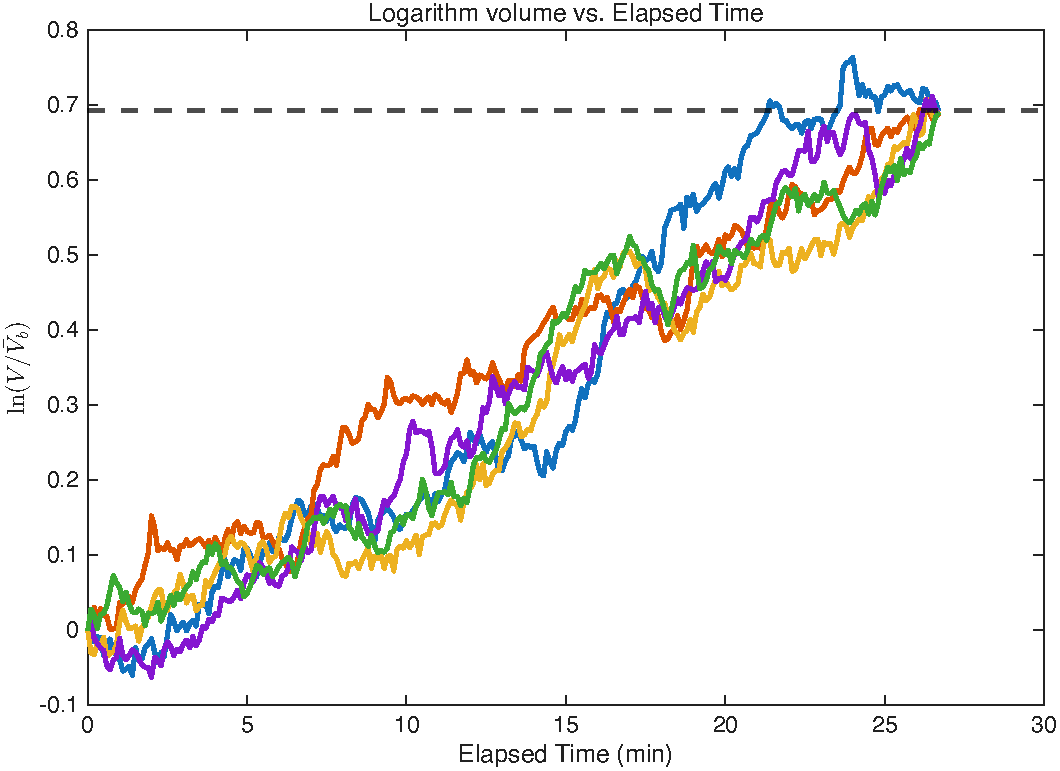
\includegraphics[width=0.65\textwidth]{appendixA.pdf}
    \caption{Five logarithmic-volume trajectories starting at $0$. The figure shows that the blue trajectory reaches the division threshold ($\ln 2$) prematurely, so it is not counted when we calculate the average growth rate for cell-volume trajectories with a doubling time of 26.7 min.}
    \label{fig:appendixA_results}
\end{figure}


{\blue To move beyond this illustrative example that focuses on a subpopulation with a particular doubling time, we now generalize this discussion to encompass the continuous distribution of varying doubling times.} In the following, we present a detailed mathematical derivation for the average growth rate in the relative-age statistics. Mathematically, the doubling time distribution can be modeled as a first-passage time problem of a drifted Brownian motion, Eq. (1) in the main text.

Cell growth involves a logarithmic volume $x$ starting at $x_0 = 0$ at $t=0$, which stops (cell division occurs) when the logarithmic volume reaches the threshold $x_{\text{div}} = \ln2$. We introduce the relative age $\phi \in [0, 1]$ as the ratio of elapsed time $t$ to the doubling time $T$:
\begin{equation}
	\phi = \frac{t}{T}.
\end{equation}
The curve in Fig.~\ref{fig:trajectory}(a) is obtained by computing the average growth rate $\lambda(\phi)$ over all cell cycles conditioned on the relative age $\phi$. To find $\lambda(\phi)$, we decompose it into two subproblems:
\begin{enumerate}
	\item Finding the doubling time distribution $P(T)$: derive the probability distribution of doubling time $P(T)$ for the biased Brownian motion, Eq. (1) in the main text.
	\item Finding the conditional average growth rate $\lambda(\phi | T)$: determine the average growth rate for all cell cycles that share the same doubling time $T$.
\end{enumerate}
${\lambda(\phi)}$ is then obtained as
\begin{equation}
	\lambda(\phi) = \int_0^\infty \lambda(\phi | T) P(T) \mathrm{d}T.
\end{equation}

\subsubsection{a. Doubling time distribution}

{\blue We define $p(x, t | x_0, 0)$ as the transition probability density of finding the logarithmic volume at $x$ at time $t$, given that it started at $x_0 = 0$ at time $t = 0$, subject to the absorbing boundary condition at $x_{\text{div}} = \ln 2$, i.e., $p(\ln 2, t | x_0, 0) = 0$. The transition probability density $p(x, t | x_0, 0)$ satisfies the forward Fokker-Planck equation (FFPE) \cite{Gardiner2009stochastic}:
\begin{equation}
\frac{\partial}{\partial t} p(x, t | x_0, 0) = -a \frac{\partial}{\partial x} p(x, t | x_0, 0) + \frac{1}{2} b^2 \frac{\partial^2}{\partial x^2} p(x, t | x_0, 0),
\label{eq:ffpe}
\end{equation}
with the point-source initial condition $p(x, 0 | x_0, 0) = \delta(x - x_0)$ and the absorbing boundary condition $p(\ln 2, t | x_0, 0) = 0$.

By applying the method of images for a drifted Brownian motion, {\blue we place an image source at $x_{\text{img}} = 2\ln 2 - x_0$ to satisfy the boundary condition.} For a general starting position $x_0 < \ln 2$, $p(x, t \mid x_0, 0)$ is explicitly solved as:
\begin{equation}
p(x, t | x_0, 0) = \frac{1}{\sqrt{2\pi b^2 t}} \left[ e^{-\frac{(x - x_0 - at)^2}{2b^2 t}} - e^{\frac{2a(\ln 2 - x_0)}{b^2}} e^{-\frac{(x - 2\ln 2 + x_0 - at)^2}{2b^2 t}} \right].
\end{equation}
Setting the initial logarithmic volume to $x_0 = 0$, the expression simplifies to:
\begin{equation}
p(x, t | 0, 0) = \frac{1}{\sqrt{2\pi b^2 t}} \left[ e^{-\frac{(x - at)^2}{2b^2 t}} - 2^{\frac{2a}{b^2}} e^{-\frac{(x - 2\ln 2 - at)^2}{2b^2 t}} \right].
\label{eq:p_transition}
\end{equation}

The probability density function $P(T)$ of the cell doubling time (i.e., the first-passage time to the division threshold $x_{\text{div}} = \ln 2$) is equivalent to the outgoing probability flux $J(x_{\text{div}}, T)$ across the absorbing boundary:
\begin{equation}
P(T) = J(\ln 2, T) = \left. \left( a p(x, T | 0, 0) - \frac{1}{2} b^2 \frac{\partial}{\partial x} p(x, T | 0, 0) \right) \right|_{x = \ln 2}.
\end{equation}
Due to the absorbing boundary condition $p(\ln 2, T | 0, 0) = 0$, the advective component vanishes at the boundary, reducing the probability flux strictly to the spatial diffusion gradient:
\begin{equation}
P(T) = -\left. \frac{1}{2} b^2 \frac{\partial}{\partial x} p(x, T | 0, 0) \right|_{x = \ln 2}.
\label{eq:flux_def}
\end{equation}

Differentiating Eq.~(\ref{eq:p_transition}) with respect to $x$ and evaluating at $x = \ln 2$ yields:
\begin{equation}
\left. \frac{\partial}{\partial x} p(x, T | 0, 0) \right|_{x = \ln 2} = -\frac{2\ln 2}{b^2 T \sqrt{2\pi b^2 T}} e^{-\frac{(\ln 2 - aT)^2}{2b^2 T}}.
\end{equation}
Substituting this spatial derivative into Eq.~(\ref{eq:flux_def}), we obtain the exact analytical expression for the doubling time distribution $P(T)$:
\begin{equation}
P(T) = \frac{\ln 2}{\sqrt{2\pi b^2 T^3}} e^{-\frac{(\ln 2 - aT)^2}{2b^2 T}}.
\label{eq:P_final}
\end{equation}

\subsubsection{b. Conditional average growth rate}
We introduce $p_1(x, t)$ as the forward probability density distribution of all trajectories starting from $x(0) = 0$ and remaining below the division threshold $\ln 2$ up to time $t$. Notice that $p_1(x, t)$ is precisely the transition probability density $p(x, t \mid 0, 0)$ derived in Eq.~(\ref{eq:p_transition}):
\begin{equation}
p_1(x, t) = \frac{1}{\sqrt{2\pi b^2 t}} \left[ e^{-\frac{(x-at)^2}{2b^2 t}} - 2^{\frac{2a}{b^2}} e^{-\frac{(x-2\ln 2-at)^2}{2b^2 t}} \right].
\label{eq:p1_sol}
\end{equation}

We next introduce $p_2(x, t)$ as the probability density distribution of all trajectories ending exactly at $t = T, x = \ln 2$ and remaining below $\ln 2$ at all times $t < T$. $p_2(x, t)$ satisfies the backward Fokker-Planck equation (BFPE) \cite{Gardiner2009stochastic}:
\begin{equation}
\frac{\partial}{\partial t}p_2(x, t) = -a\frac{\partial}{\partial x}p_2(x, t) - \frac{1}{2}b^2\frac{\partial^2}{\partial x^2}p_2(x, t),
\end{equation}
with the initial condition set at the final state $p_2 (x, T) = \delta(x-\ln 2)$ and the boundary condition $p_2 (\ln 2, t) = 0$. We find that $p_2(x, t)$ has the following property:
\begin{equation}
p_2 (x, t) \propto \frac{1}{\sqrt{2\pi b^2 (T-t)}} \frac{\ln 2 - x}{T-t} e^{-\frac{(\ln 2 - x - a(T-t))^2}{2b^2 (T-t)}}.
\label{eq:p2_sol}
\end{equation}
}

We next introduce the probability density function $p(x, t|T)$ of all trajectories that start at $x=0$ at $t=0$ and reach the division threshold $x=\ln 2$ the first time at $t=T$, which is related to $p_1$ and $p_2$ by
\begin{equation}
	p(x, t|T) \propto p_1 (x, t) p_2 (x, t).
	\label{eq:conditional_density}
\end{equation}
Obviously, when $x \ge \ln 2$, $p(x, t|T) = 0$. We next compute the average position $x(t)$ at time $t$ over $p(x, t|T)$
\begin{equation}
	x(t|T) = \frac{\int_{-\infty}^{\ln 2} x p(x, t|T) \mathrm{d}x}{\int_{-\infty}^{\ln 2} p(x, t|T) \mathrm{d}x},
	\label{eq:x_avg_def}
\end{equation}
where $p(x, t|T)$ is the conditional probability density function. The analytical solution for $x(t|T)$ turns out to be
\begin{equation}
	x(t|T) = \ln 2 - \left[ \left( (1-\frac{t}{T})\ln 2 + \frac{b^2 t}{\ln 2} \right) \operatorname{erf}\left( \ln 2\sqrt{\frac{T-t}{2b^2 tT}} \right) + \sqrt{\frac{2b^2 (T-t)t}{\pi T}} e^{-\frac{(\ln 2)^2 (T-t)}{2b^2 Tt}} \right].
	\label{eq:x_avg_sol}
\end{equation}
The conditional average growth rate $\lambda(t|T)$ is the time derivative of the average position: $\lambda(t|T) = \frac{\mathrm{d}x(t|T)}{\mathrm{d}t}$, which is 
\begin{equation}
	\lambda(t|T) = \left( \frac{\ln 2}{T} - \frac{b^2}{\ln 2} \right) \operatorname{erf}\left( \ln 2\sqrt{\frac{T-t}{2b^2 tT}} \right) + \sqrt{\frac{2t b^2}{\pi T(T-t)}} e^{-\frac{(\ln 2)^2 (T-t)}{2b^2 Tt}}.
	\label{eq:x_prime_sol}
\end{equation}



 %The solution represents a zero-measure set (if you consider a rigorous solution), but it does not preclude the existence of a probability distribution.
%The average normalized growth rate trajectory, $\lambda(t | T)$, is obtained by differentiating the conditional expected position, $x(t | T)$, where the expected position is calculated through the spatial integration of the logarithmic volume $x$ against the conditional probability density $p(x, t | T)$. Finally, $\lambda(t|T)$ is normalized to the time scale $\phi \in [0, 1]$ to yield $\lambda(\phi | T)$.




We next convert the conditional average growth rate $\lambda(t|T)$ as a function of the relative age $\phi \in [0, 1]$ by substituting $t = \phi T$:
\begin{equation}
\lambda(\phi | T) = \left( \frac{\ln 2}{T} - \frac{b^2}{\ln 2} \right) \operatorname{erf}\left( \ln 2 \sqrt{\frac{1-\phi}{2b^2 \phi T}} \right) + \sqrt{\frac{2\phi b^2}{\pi T(1-\phi)}} e^{-\frac{(\ln 2)^2 (1-\phi)}{2b^2 \phi T}}.
\label{eq:conditional_rate}
\end{equation}

The average growth rate $\lambda(\phi)$ over all cell cycles conditioned on the relative age $\phi$ is obtained by integrating the conditional average growth rate $\lambda(\phi | T)$ with the doubling time distribution $P(T)$ over $T$:
\begin{equation}
\lambda(\phi) = \int_0^{+\infty} \frac{\ln 2}{\sqrt{2\pi b^2 T^3}} e^{-\frac{(\ln 2 - aT)^2}{2b^2 T}} \left[ \left( \frac{\ln 2}{T} - \frac{b^2}{\ln 2} \right) \operatorname{erf}\left( \ln 2\sqrt{\frac{1-\phi}{2b^2 \phi T}} \right) + \sqrt{\frac{2\phi b^2}{\pi T(1-\phi)}} e^{-\frac{(\ln 2)^2 (1-\phi)}{2b^2 \phi T}} \right] \mathrm{d}T.
\label{eq:final_integral_composite}
\end{equation}
We confirm the validity of Eq.~(\ref{eq:final_integral_composite}) by comparing it with direct numerical simulations similar to Fig.~1 in the main text except the birth and division volumes are fixed at $V_b=1$ and $V_d=2$ (Fig.~\ref{fig:asymptotic_results}).

\begin{figure}[htb!]
    \centering
    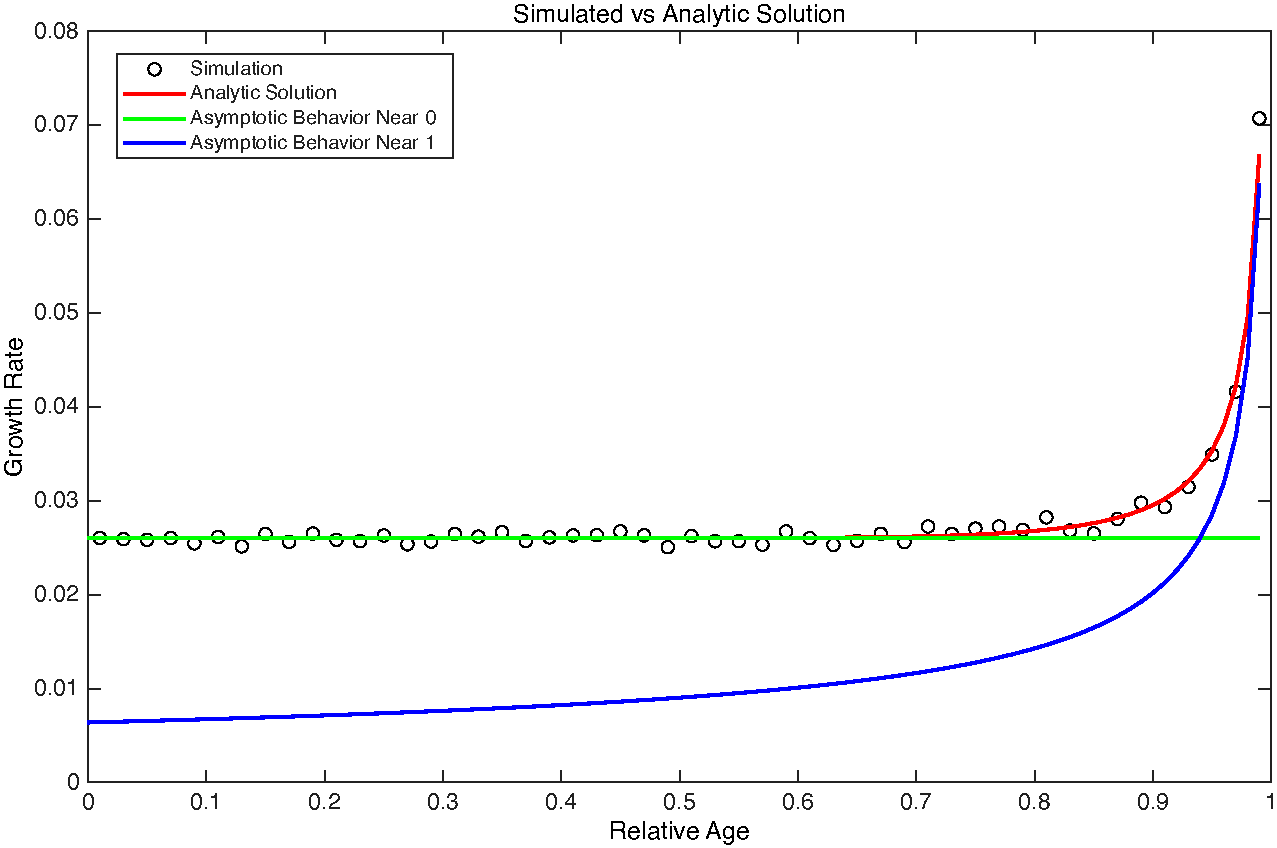
\includegraphics[width=0.9\textwidth]{asymptotic.pdf}
    \caption{The theoretical prediction Eq.~(\ref{eq:final_integral_composite}) agrees with the numerical simulation. We also show the predicted asymptotic behaviors near $\phi \to 0$ and $\phi \to 1$.}
    \label{fig:asymptotic_results}
\end{figure}

In the limit where the relative age $\phi\rightarrow 0$, the average growth rate approaches the deterministic growth rate $a$:
\begin{equation}
\lim_{\phi \to 0} \lambda(\phi) \approx \int_0^{+\infty} \frac{\ln 2}{\sqrt{2\pi b^2 T^3}} e^{-\frac{(\ln 2 - aT)^2}{2b^2 T}} \left( \frac{\ln 2}{T} - \frac{b^2}{\ln 2} \right) \mathrm{d}T = a.
\label{lim at 0}
\end{equation}

In the limit where $\phi\rightarrow 1$, the error function term tends to zero and the average growth rate turns out to be
\begin{equation}
\lim_{\phi \to 1} \lambda(\phi) \approx \frac{2a}{\pi\sqrt{1-\phi}} 2^{a/b^2} K_1 \left( \frac{a \ln 2}{b^2} \right),
\label{lim at 1}
\end{equation}
where $K_1(x)$ is the modified Bessel function of the second kind of order one. This analysis reveals a critical finding: as $\phi \to 1$, the average normalized growth rate $\lambda(\phi)$ diverges with the asymptotic form:
\begin{equation}
\lambda(\phi) \propto \frac{1}{\sqrt{1-\phi}}.
\label{divergent exponent}
\end{equation}

%To estimate the range where this selection bias ($\phi \to 1$ divergence) dominates, we define the boundary range by the intersection point where the asymptotic solution $\lambda(\phi)|_{\phi \to 1}$ equals $a$. By equating the two asymptotic solutions, the intersection point $1-\phi$ is found to be:
%\begin{equation}
%	1 - \phi \approx \left[ \frac{2}{\pi} 2^{a/b^2} K_1 \left( \frac{a \ln 2}{b^2} \right) \right]^2 \equiv f\left( \frac{a}{b^2} \right).
%	\label{eq:boundary_range}
%\end{equation}
%The function $f(a/b^2)$ is a monotonically decreasing function of the ratio $a/b^2$. {\blue This functional dependence implies that {\red this dimensionless number locally modulates the boundary effect. We note that even if} the deterministic growth rate ($a$) and the noise intensity ($b$) dynamically depend on the cell cycle (e.g., via the cell volume), the divergence exponent near the cell-cycle end ($\phi \to 1$) remains robustly fixed at $0.5$, as the local first-passage dynamics inevitably dominate the boundary-crossing physics.}

%This indicates that the shape and range of the boundary effect are entirely governed by the single dimensionless parameter $\frac{a}{b^2}$. This dependency is fundamentally consistent with the structure of the initial SDE Eq.~(ref{SDE equation}).

%The solution of this linear SDE is inherently scalable and dependent only on the ratio of the drift term ($a$) to the noise strength ($b^2$).





%Furthermore, if the underlying growth fluctuation were not a standard Wiener process but exhibited long-range correlation described by Hurst Exponent ($H$), the resulting divergence exponent ($\gamma$) would be generalized as:
%\begin{equation}
%\gamma = 1 - H
%\label{eq:hurst_exponent_divergence}
%\end{equation}
%This demonstrates how the memory properties of the noise ($H \neq 0.5$) would modify the exponent of the divergence observed in the system's rate.

{\blue
\subsection{III. Microscopic mapping of experimental perturbations}

In the following, we apply the perturbations introduced in the paper by Basan's lab~\cite{Mukherjee2025bacterial} to our model and discuss the corresponding experimental expectations.

\paragraph{1. MepS Titration.}
Endopeptidase (MepS) titration alters the rates of enzymatic crosslink cleavage and material addition, thereby modulating the effective viscosity of the growth dashpot ($\eta_0$). Crucially, this process does not change the crosslinking density or local stiffness of the cell wall. Therefore, the micro-viscoelastic parameters ($\eta, E_i$) remain unchanged. We emphasize that while the growth viscosity $\eta_0$ is an effective value determined by the time scale of crosslink cleavage, the micro-viscosity $\eta$ is a material property independent of cell growth.

Given these conditions, we predict that upon MepS titration, the deterministic growth rate $a = \bar{\sigma} / \eta_0$ varies as observed in experiments from Basan's Lab~\cite{Mukherjee2025bacterial}; however, the variance of the logarithmic volume change $\sigma_x^2(\Delta t)$, including the scaling exponent, remains unchanged.

\paragraph{2. Ampicillin Treatment.}
Ampicillin compromises the structural integrity of the pre-existing peptidoglycan network by reducing its crosslinking density. We model the effects of ampicillin as a global softening of all Voigt elements, i.e., $E_i' = f E_i$ where the factor $f < 1$. Since $\tau_i = \eta / E_i$, ampicillin increases the relaxation times globally. In terms of the power-law distribution of relaxation times $P(\tau) = C \tau^{-\beta}$, this means a larger lower bound $\tau_0' = \tau_0 / f$ and a larger prefactor $C' = C / f^{\beta - 1}$.

Recall that the variance of logarithmic volume increment, i.e., the mean square displacement (MSD) of $x(t)$, has the following expression:
\begin{equation}
    \sigma_x^2(\Delta t) \propto C^2 A_\sigma \Delta t^{3 - 2\beta} \quad \text{(see Eq.~(9) in the main text)},
\end{equation}
Thus, we predict that our conclusions about subdiffusive random growth remain unchanged, but with a larger prefactor in the MSD. Here, we assume the noise amplitude of the cell wall tension $A_\sigma$ is constant. We note that ampicillin treatment reduces the turgor pressure, which may lead to a lower noise amplitude $A_\sigma$. If this is the case, we expect the amplification of the MSD to be offset by a lower $A_\sigma$.

\paragraph{3. Modulating Cell Width.}
Increasing cell width, e.g., by inhibiting MreB, increases cell wall tension at constant turgor pressure, given the relationship $\sigma = r P / 2d$. Interestingly, experiments from Basan's Lab~\cite{Mukherjee2025bacterial} found that the increase in cell width is compensated by lower turgor pressure and biomass density. Thus, we expect cell wall tension to be approximately constant, implying a constant $A_\sigma$. Therefore, regarding the MSD of $x(t)$, we predict it to be the same as in wild-type cells.

}

{\blue
\subsection{IV. Derivation of the subdiffusive exponent in the viscoelastic model}

In the main text, we model the cell wall as a complex viscoelastic material where the relaxation times of the internal Voigt elements follow a power-law distribution, $P(\tau) = C\tau^{-\beta}$. In the following, we derive Eq. (9) in the main text.


As given by Eq.~(8) in the main text, the overall growth noise $\xi(t)$ is expressed as the convolution:
\begin{equation}
	\xi(t) = C \int_0^{\infty} \mathrm{d}g \, g^{1-\beta} F(g/\tau_0) \delta \sigma(t-g),
\end{equation}
where $\delta \sigma(t)$ represents the white noise tension fluctuations satisfying $\langle \delta \sigma(t_1) \delta \sigma(t_2) \rangle = 2A_{\sigma} \delta(t_1 - t_2)$.

The mean square displacement (MSD) over a time interval $\Delta t$ is calculated by  $\sigma_x^2(\Delta t) = \langle [\xi(\Delta t) - \xi(0)]^2 \rangle$. Substituting the expression for $\xi(t)$, the stochastic increment is:
\begin{equation}
	\xi(\Delta t) - \xi(0) = C \int_0^{\infty} \mathrm{d}g \, g^{1-\beta} F(g/\tau_0) [\delta \sigma(\Delta t - g) - \delta \sigma(-g)].
\end{equation}

We next compute the variance $\sigma_x^2(\Delta t) = \langle [\xi(\Delta t) - \xi(0)]^2 \rangle$ as
\begin{equation}
	\sigma_x^2(\Delta t)= C^2 \int_0^{\infty} \mathrm{d}g_1 \int_0^{\infty} \mathrm{d}g_2 \, g_1^{1-\beta} F(g_1/\tau_0) g_2^{1-\beta} F(g_2/\tau_0) \langle (\delta \sigma(\Delta t - g_1) - \delta \sigma(-g_1)) (\delta \sigma(\Delta t - g_2) - \delta \sigma(-g_2)) \rangle,
\end{equation}
%where we have defined the shorthand $\mathcal{K}(g) = g^{1-\beta} F(g/\tau_0)$ and the noise increment $\Delta\delta \sigma(g) = \delta \sigma(\Delta t - g) - \delta \sigma(-g)$.

Using the white noise correlation $\langle \delta \sigma(t_1) \delta \sigma(t_2) \rangle = 2A_{\sigma}\delta(t_1 - t_2)$, we obtain
\begin{equation}
	\sigma_x^2(\Delta t) = 4C^2 A_{\sigma}\int_0^{\infty} \mathrm{d}g \Bigl\{ \left[ g^{1-\beta} F\left(\frac{g}{\tau_0}\right) \right]^2- (\Delta t + g)^{1-\beta} g^{1-\beta} F\left(\frac{g}{\tau_0}\right) F\left(\frac{\Delta t + g}{\tau_0}\right)\Bigl\}.
\end{equation}

%the expansion of $[\delta \sigma(\Delta t - g_1) - \delta \sigma(-g_1)][\delta \sigma(\Delta t - g_2) - \delta \sigma(-g_2)]$ generates four terms that are evaluated via the $\delta$-functions: the two self-correlations each yield 
%\begin{equation}
%2A_{\sigma} \int_0^{\infty} \mathrm{d}g_1 \, \left[ g_1^{1-\beta} F\left(\frac{g_1}{\tau_0}\right) \right]^2,
%\end{equation}
%while the cross-correlations contribute
%\begin{equation}
%-4A_{\sigma} \int_0^{\infty} \mathrm{d}g_1 \, (\Delta t + g_1)^{1-\beta} g_1^{1-\beta} F\left(\frac{g_1}{\tau_0}\right) F\left(\frac{\Delta t + g_1}{\tau_0}\right).
%\end{equation}

%Combining these contributions and renaming the dummy integration variable $g_1$ to $g$, we directly arrive at the explicit integral expression:

%To extract the temporal scaling $\Delta t^{3-2\beta}$ and recover Eq.~(9), 

%which implies $g = \Delta t / u$ and $\mathrm{d}g = -(\Delta t / u^2) \mathrm{d}u$. Applying this substitution to the squared term yields:
%\begin{equation}
%	g^{2-2\beta} \mathrm{d}g = -\left(\frac{\Delta t}{u}\right)^{2-2\beta} \frac{\Delta t}{u^2} \mathrm{d}u = -\Delta t^{3-2\beta} u^{2\beta-4} \mathrm{d}u,
%\end{equation}
%and identically for the cross-term:
%\begin{equation}
%	(\Delta t + g)^{1-\beta} g^{1-\beta} \mathrm{d}g = -\left(\Delta t + \frac{\Delta t}{u}\right)^{1-\beta} \left(\frac{\Delta t}{u}\right)^{1-\beta} \frac{\Delta t}{u^2} \mathrm{d}u = -\Delta t^{3-2\beta} u^{2\beta-4} (1+u)^{1-\beta} \mathrm{d}u.
%\end{equation}
%The arguments of the incomplete gamma functions transform as $g/\tau_0 = \Delta t / (u \tau_0)$ and $(\Delta t + g)/\tau_0 = \Delta t/\tau_0 + \Delta t / (u \tau_0)$.

Finally, we introduce the integration variable $u = \Delta t / g$ and obtain the MSD of the logarithmic volume as
\begin{equation}
	\sigma_x^2(\Delta t) =4C^2A_{\sigma} \Delta t^{3-2\beta} \int_0^\infty u^{2\beta-4} \left[ F\left(\frac{\Delta t}{u\tau_0}\right)^2 - (1+u)^{1-\beta} F\left(\frac{\Delta t}{u\tau_0}\right) F\left(\frac{\Delta t}{u\tau_0} + \frac{\Delta t}{\tau_0}\right) \right] du 
	\label{msd}
\end{equation}

Clearly, for the probability distribution of the relaxation time to be normalizable, we require $\beta>1$. Below, we discuss the value of the subdiffusive exponent considering two different regimes of $\beta$.

%The scaling behavior of the mean square displacement (MSD) of the logarithmic volume, $\sigma_x^2(\Delta t)$, depends critically on the value of the exponent $\beta$. 


%\subsubsection{The unphysical regime $\beta < 1$}
%The relaxation time $\tau$ follows a power-law distribution with a microscopic lower bound $\tau_0$. For $P(\tau)$ to be a mathematically valid probability density function, it must be normalizable:
%\begin{equation}
%\int_{\tau_0}^{\infty} P(\tau) d\tau = C \int_{\tau_0}^{\infty} \tau^{-\beta} d\tau = 1 
%\end{equation}
%Evaluating the indefinite integral yields:
%\begin{equation}
%\int_{\tau_0}^{\infty} \tau^{-\beta} d\tau = \lim_{\tau_{max} \to \infty} \left[ \frac{\tau^{1-\beta}}{1-\beta} \right]_{\tau_0}^{\tau_{max}} 
%\end{equation}
%If $\beta < 1$, the exponent $1-\beta$ is positive. Consequently, as $\tau_{max} \to \infty$, the term $\tau_{max}^{1-\beta}$ unconditionally diverges to infinity, making it impossible to normalize the distribution. Therefore, to define a physical relaxation-time distribution, we must strictly require $\beta > 1$, which subsequently yields the exact normalization factor $C = (\beta-1)\tau_0^{\beta-1}$ introduced in the main text.

\subsubsection{a. The subdiffusive regime $1 < \beta < 3/2$}

To establish the subdiffusive scaling, we evaluate the integral in Eq. (\ref{msd}) in the long-time limit $\Delta t / \tau_0 \gg 1$ and show that it is a finite value. In this asymptotic regime, one can replace $F(x) = \int_0^x v^{\beta-2} e^{-v} dv$ by its asymptotic value $F(x) \to \Gamma(\beta-1)$ as $x \to \infty$ according to Lebesgue dominated convergence theorem, such that the bracketed term in the integrand safely simplifies to
\begin{equation}
\Gamma(\beta-1)^2 \left[ 1 - (1+u)^{1-\beta} \right] 
\end{equation}
Thus, the integral in Eq. (\ref{msd}) behaves proportionally to:
\begin{equation}
I = \int_0^\infty u^{2\beta-4} \left[ 1 - (1+u)^{1-\beta} \right] du 
\end{equation}
For the $\Delta t^{3-2\beta}$ power law to strictly hold, this integral $I$ must converge to a finite constant. We analyze its asymptotic behavior at both integration boundaries: Using the Taylor expansion for infinitesimally small $u$, we have $(1+u)^{1-\beta} \approx 1 - (\beta-1)u$. The integrand thus behaves as $u^{2\beta-4} \cdot (\beta-1)u \propto u^{2\beta-3}$. For the integral to converge at the lower bound, we require the exponent to be strictly greater than $-1$ (i.e., $2\beta-3 > -1$), which simplifies to $\beta > 1$. For sufficiently large $u$, the term $(1+u)^{1-\beta} \to 0$ given $\beta > 1$. The integrand therefore directly scales as $u^{2\beta-4}$. For convergence at the upper bound, we require the exponent to be strictly less than $-1$ (i.e., $2\beta-4 < -1$), which yields $\beta < 3/2$.

Because both boundary conditions are simultaneously satisfied exclusively within the range $1 < \beta < 3/2$, the integral does not diverge at either end and successfully evaluates to a finite constant. As a result, the MSD accurately follows the power-law scaling $\sigma_x^2(\Delta t) \sim \Delta t^\alpha$ with the expected subdiffusive exponent $\alpha = 3 - 2\beta$.

\subsubsection{b. The stationary regime $\beta > 3/2$}

To study the $\beta > 3/2$ regime, we introduce a change of variables, $v = \frac{\Delta t}{u\tau_0}$. Substituting $u = \frac{\Delta t}{v\tau_0}$ into Eq. (\ref{msd}), we find that 
\begin{equation}
	\sigma_x^2(\Delta t) \sim \int_0^\infty v^{2-2\beta} \left[ F(v)^2 - \left(1 + \frac{\Delta t}{v\tau_0}\right)^{1-\beta} F(v) F\left(v + \frac{\Delta t}{\tau_0}\right) \right] dv,\label{msd1}
\end{equation}
where constant factors that are independent of $\Delta t$ are not shown. We now evaluate the long-time limit $\Delta t \to \infty$ for the new integral in Eq. (\ref{msd1}). For any fixed $v$, because $\beta > 1$, the term $\left(1 + \frac{\Delta t}{v\tau_0}\right)^{1-\beta}$ asymptotically decays to zero. Consequently, the entire second term in the bracket vanishes, reducing the asymptotic integral to:
\begin{equation}
	I_v = \int_0^\infty v^{2-2\beta} F(v)^2 dv.
\end{equation}
For this integral $I_v$ to evaluate to a finite value, it must converge at both boundaries. 

The incomplete Gamma function behaves as $F(v) \approx \frac{v^{\beta-1}}{\beta-1}$ at the lower bound. Thus, the integrand scales as $v^{2-2\beta} \cdot v^{2\beta-2} = v^0 = 1$ and it converges at the lower bound for all $\beta$. For $v\rightarrow \infty$, $F(v)$ converges to the constant $\Gamma(\beta-1)$ as $v \to \infty$. Therefore, the integrand scales asymptotically as $v^{2-2\beta}$. For this tail to be integrable, we require the exponent to be less than $-1$ (i.e., $2 - 2\beta < -1$), which directly yields the condition $\beta > 3/2$. Therefore, for $\beta > 3/2$, the integral $I_v$ evaluates to a finite constant, which means that $\sigma_x^2(\Delta t) \sim \Delta t^{0}$.


}
\bibliography{Lin_Dec_05_2025}

%This rigorous derivation proves that for $\beta > 3/2$, the internal scaling exponent of the integral ($2\beta-3$) exactly cancels the prefactor exponent ($3-2\beta$). The overall MSD strictly saturates to a time-independent plateau ($\sigma_x^2 \sim \text{const}$), formally demonstrating that the subdiffusive power-law exponent drops to $\alpha = 0$.




%\begin{figure}[htb!]
%   \centering
%   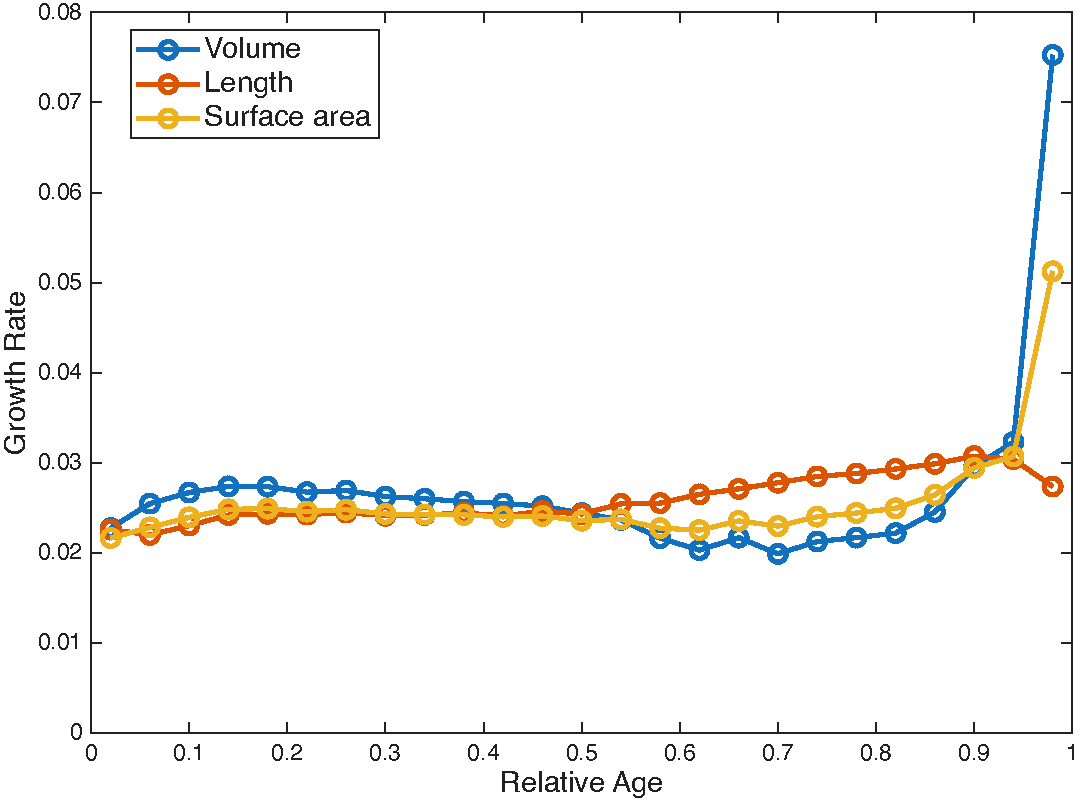
\includegraphics[width=0.6\textwidth]{surface.pdf}
%   \caption{Average growth rates of different morphological parameters (volume, surface area, and length) as a function of relative age. Calculations for cell volume and surface area follow the methods detailed in Ref.~[8]. During the first half of the cell cycle, the growth rates of the surface area and the cell length match closely. This indicates that the cell width remains relatively constant during this phase, with growth driven primarily by length extension. However, in the second half of the cell cycle, the growth-rate trajectory of the surface area deviates from that of the cell length and instead behaves much more similarly to that of the cell volume. This morphological shift suggests an active regulation of the cell radius to coordinate surface area and volume. We hypothesize that the mean growth rate of the cell is fundamentally constrained by its surface area (e.g., due to nutrient uptake capacity), which dynamically couples to the volume to sustain the widely observed exponential growth. Such a geometric transition points toward an as-yet-unidentified biological regulatory mechanism during the late cell cycle.}
%   \label{fig:surface}
%\end{figure}



\newpage
\begin{figure}[htb!]
   \centering
   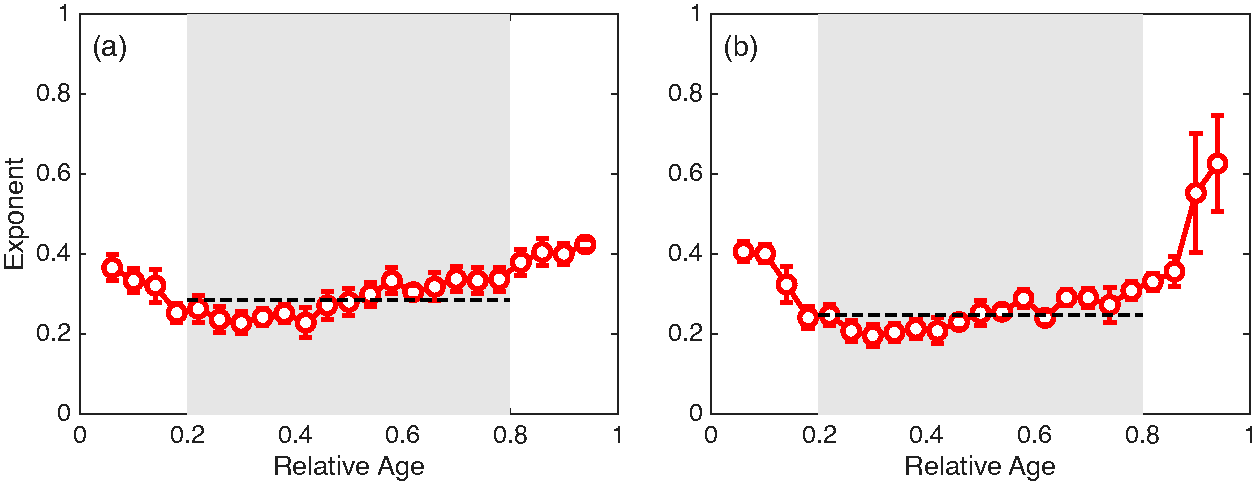
\includegraphics[width=0.8\textwidth]{LSexp.pdf}
   \caption{The same analysis as Fig.~2(f) in the main text, but for the data of cell length (a) and surface area (b).}
   \label{fig:LSexp}
\end{figure}

\begin{figure}[htb!]
	\centering
	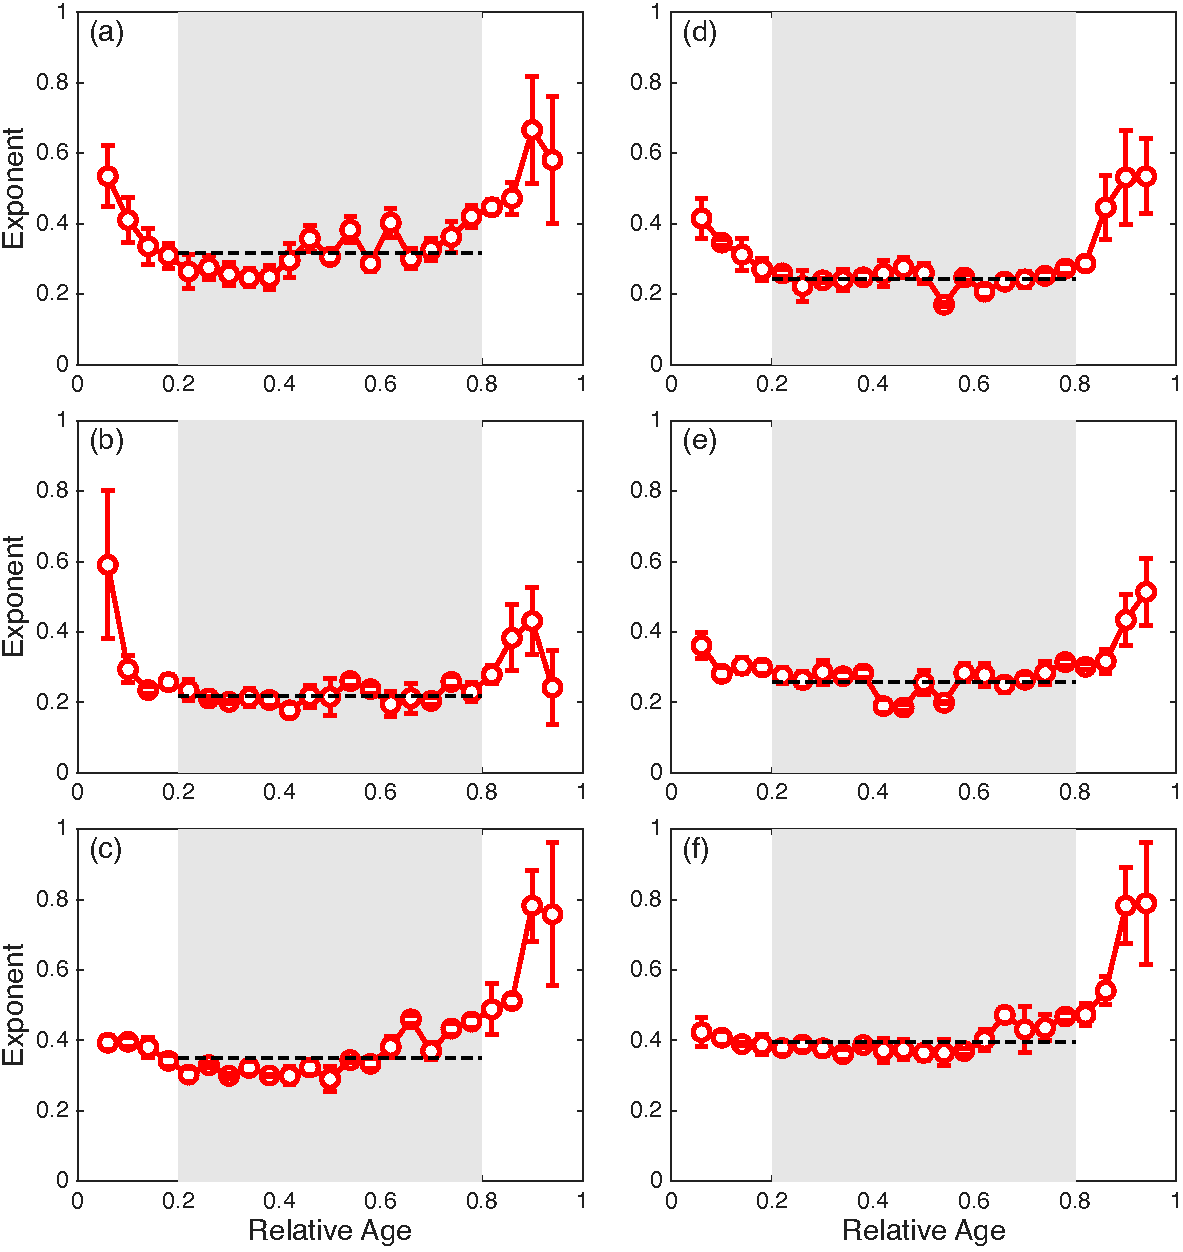
\includegraphics[width=0.8\textwidth]{robustness.pdf}
	\caption{The same analysis as Fig.~2(f) in the main text, but for different growth mediums, including (a) glucose+6 a.a, (b) glucose, (c) glycerol, (d) sorbitol, (e) synthetic rich, and (f) tryptic soy broth (TSB) according to Ref. \cite{Taheri2015cell}.}
	\label{fig:robustness}
\end{figure}

\begin{figure}[htb!]
	\centering
	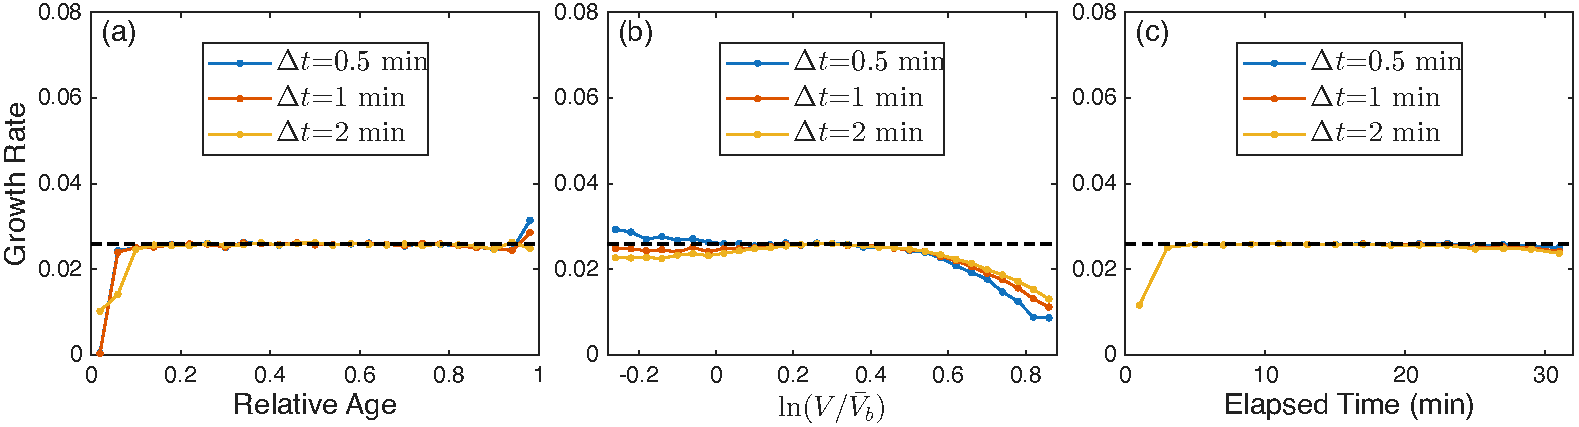
\includegraphics[width=1.0\textwidth]{colored.pdf}
	\caption{The same analysis as Fig.~\ref{fig:deltat}(a-c), but the growth rate noise is generated from the general Voigt model with $\beta=1.375$. We note that for the relative-volume statistics, the deviation from the ground truth is more significant as $\Delta t$ decreases.}
	\label{fig:colored}
\end{figure}

\begin{figure}[htb!]
	\centering
	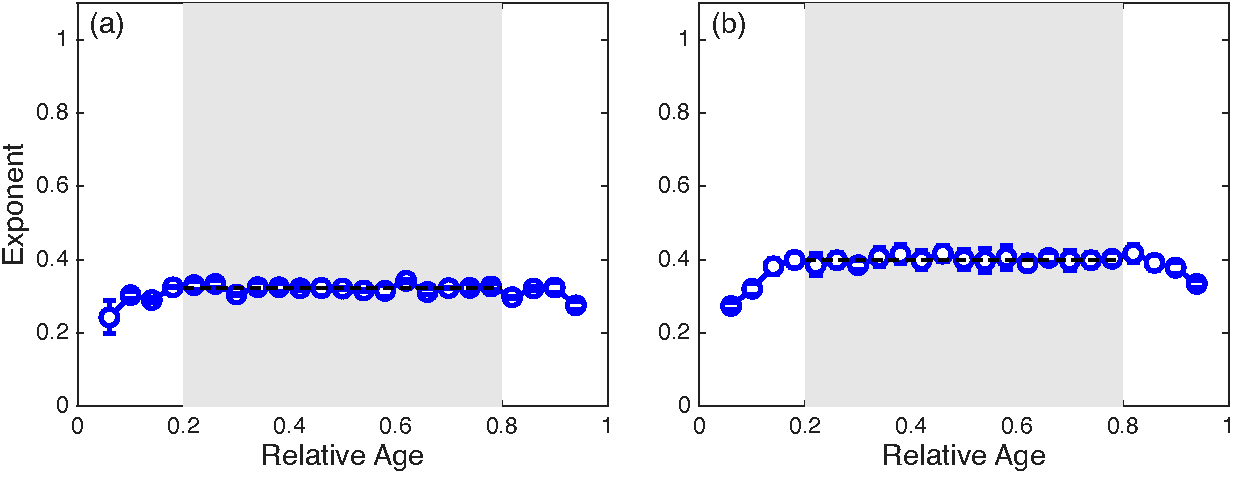
\includegraphics[width=0.8\textwidth]{variedk.pdf}
	\caption{The same analysis as in Fig.~3(g) of the main text, but for the extended model in which the deterministic growth rate is random across cell cycles. We sample the deterministic growth rate for each cell cycle from a normal distribution with mean equal to $0.026$ and the coefficient of variation equal to 0.1 in (a) and 0.2 in (b), which are biologically reasonable values \cite{Taheri2015cell}. We find that the subdiffusive random growth remains robust.}
	\label{fig:variedk}
\end{figure}

\begin{figure}[htb!]
	\centering
	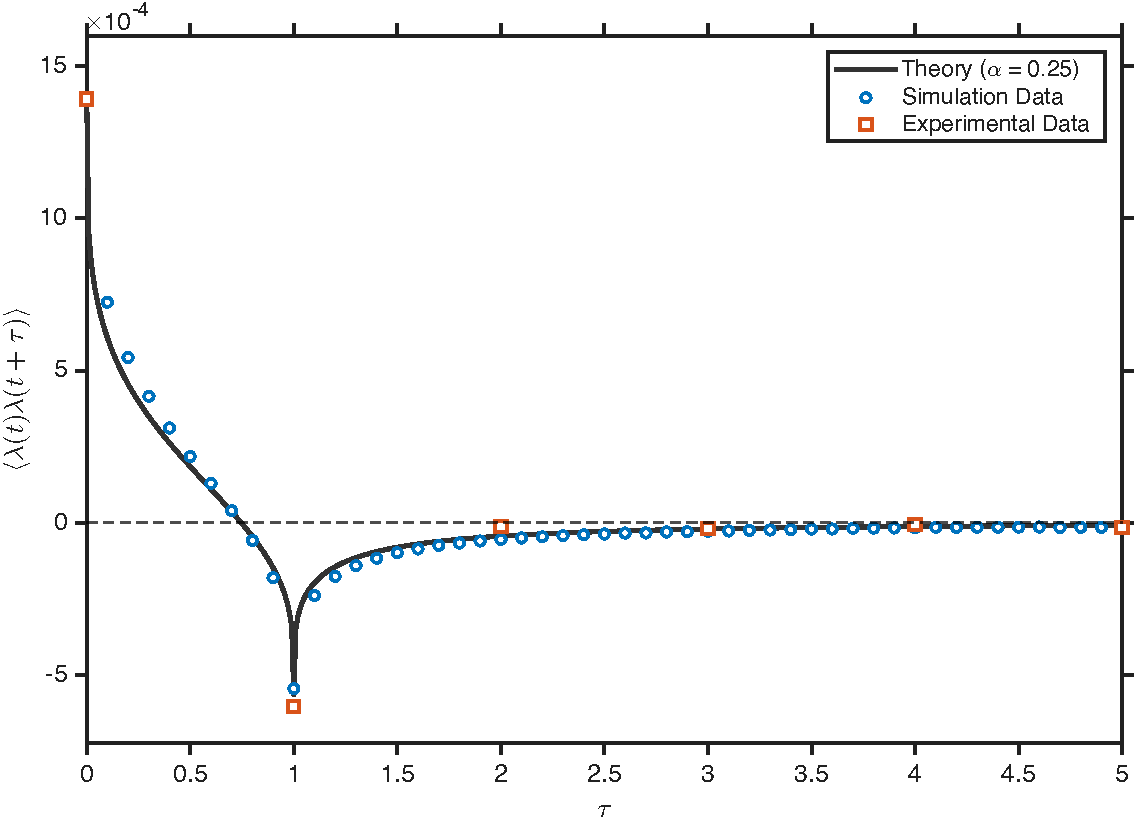
\includegraphics[width=0.8\textwidth]{correlation.pdf}
	\caption{Temporal autocorrelation function of growth rate fluctuations, $\langle \delta \lambda(t)\delta \lambda(t+\tau)\rangle$ as a function of the time lag $\tau$. Here $\delta \lambda(t)$ is computed as $(x(t+\Delta t)-x(t))/\Delta t -a $ where $\Delta t=1$ min and $a$ is the deterministic growth rate. For the experimental data, we compute $a$ for each cell cycle as $(x(T)-x(0))/T$, where $x(0)$ and $x(T)$ are the logarithmic cell volume at cell birth and division, respectively, and $T$ is the doubling time. Experimental data (red hollow squares) and numerical simulation data (blue hollow circles) are shown alongside the theoretical prediction \cite{Mandelbrot1968fractional} (black solid line, $\alpha = 0.25$). Theoretical parameters are calibrated such that the curve coincides with the experimental data at $\tau = 0$. Both experimental and simulation results show excellent agreement with the theoretical curve, capturing the pronounced negative dip at $\tau = 1$ and the subsequent long-tail negative correlation. This highlights the long-term memory effect inherent in the subdiffusive random growth of cell volume.}
	\label{fig:correlation}
\end{figure}

\begin{figure}[htb!]
	\centering
	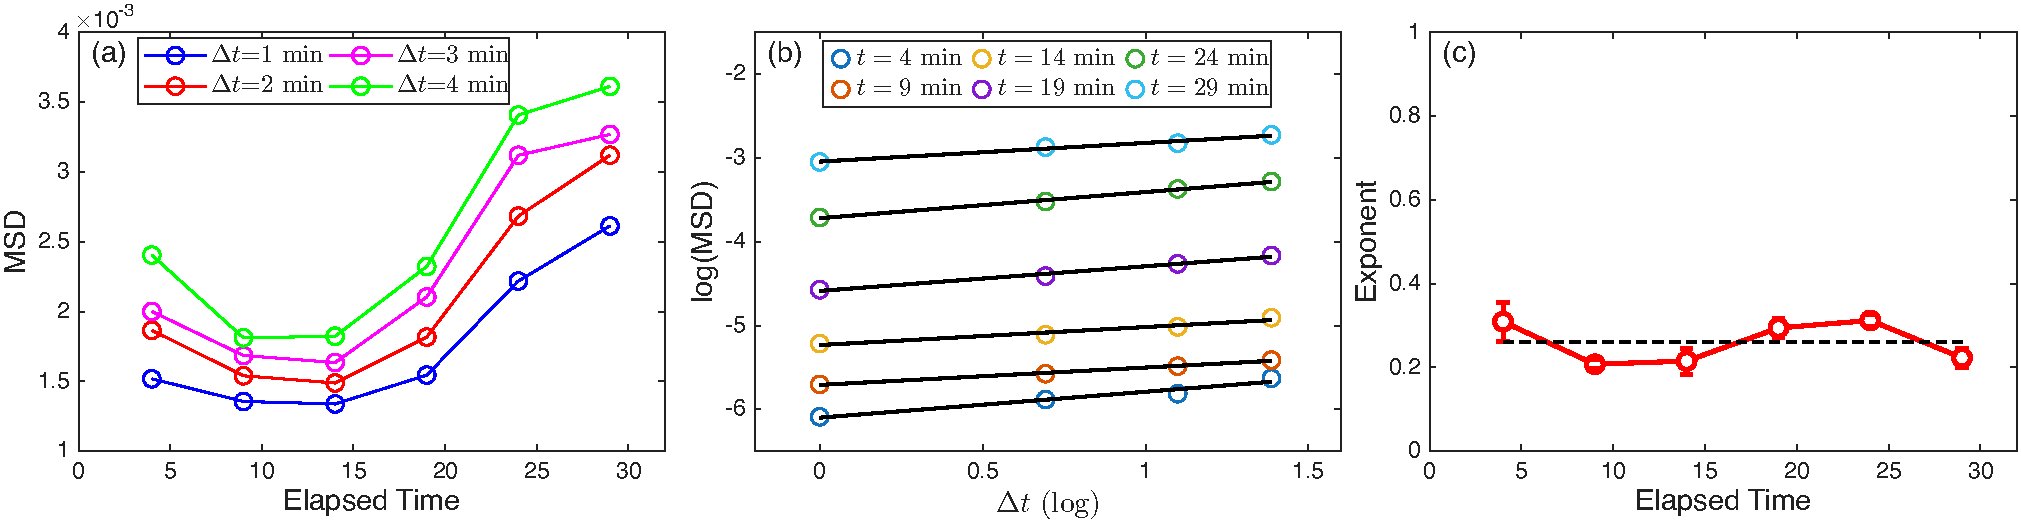
\includegraphics[width=1.0\textwidth]{timstaexp.pdf}
	\caption{The same analysis as Figure 2(d-f) in the main text but conditioned on elapsed time.}
	\label{fig:timstaexp}
\end{figure}

\begin{figure}[htb!]
	\centering
	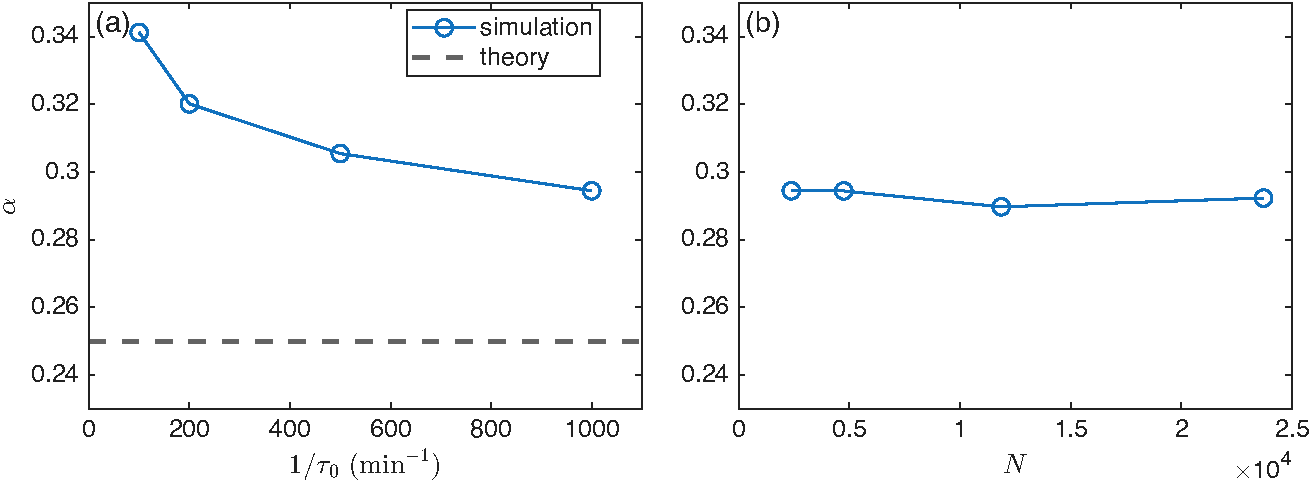
\includegraphics[width=0.8\textwidth]{expvstau.pdf}
	\caption{Dependence of the measured subdiffusive exponent $\alpha$ on the minimum relaxation time $\tau_0$ and the number of Voigt elements $N$. (a) Measured exponent $\alpha$ as a function of the inverse minimum relaxation time $1/\tau_0$ in the power-law distribution. As $\tau_0$ decreases (i.e., $1/\tau_0$ increases), the measured exponent from numerical simulations (blue circles) systematically approaches the theoretically predicted value of $0.25$ (dashed line). (b) Measured exponent $\alpha$ versus the number of Voigt elements $N$, with a fixed minimum relaxation time $\tau_0 = 0.001\text{ min}$. The measured exponent remains virtually invariant across different values of $N$, demonstrating that the subdiffusive scaling is insensitive to the maximum relaxation time cutoff.}
	\label{fig:expvstau}
\end{figure}

\begin{figure}[htb!]
	\centering
	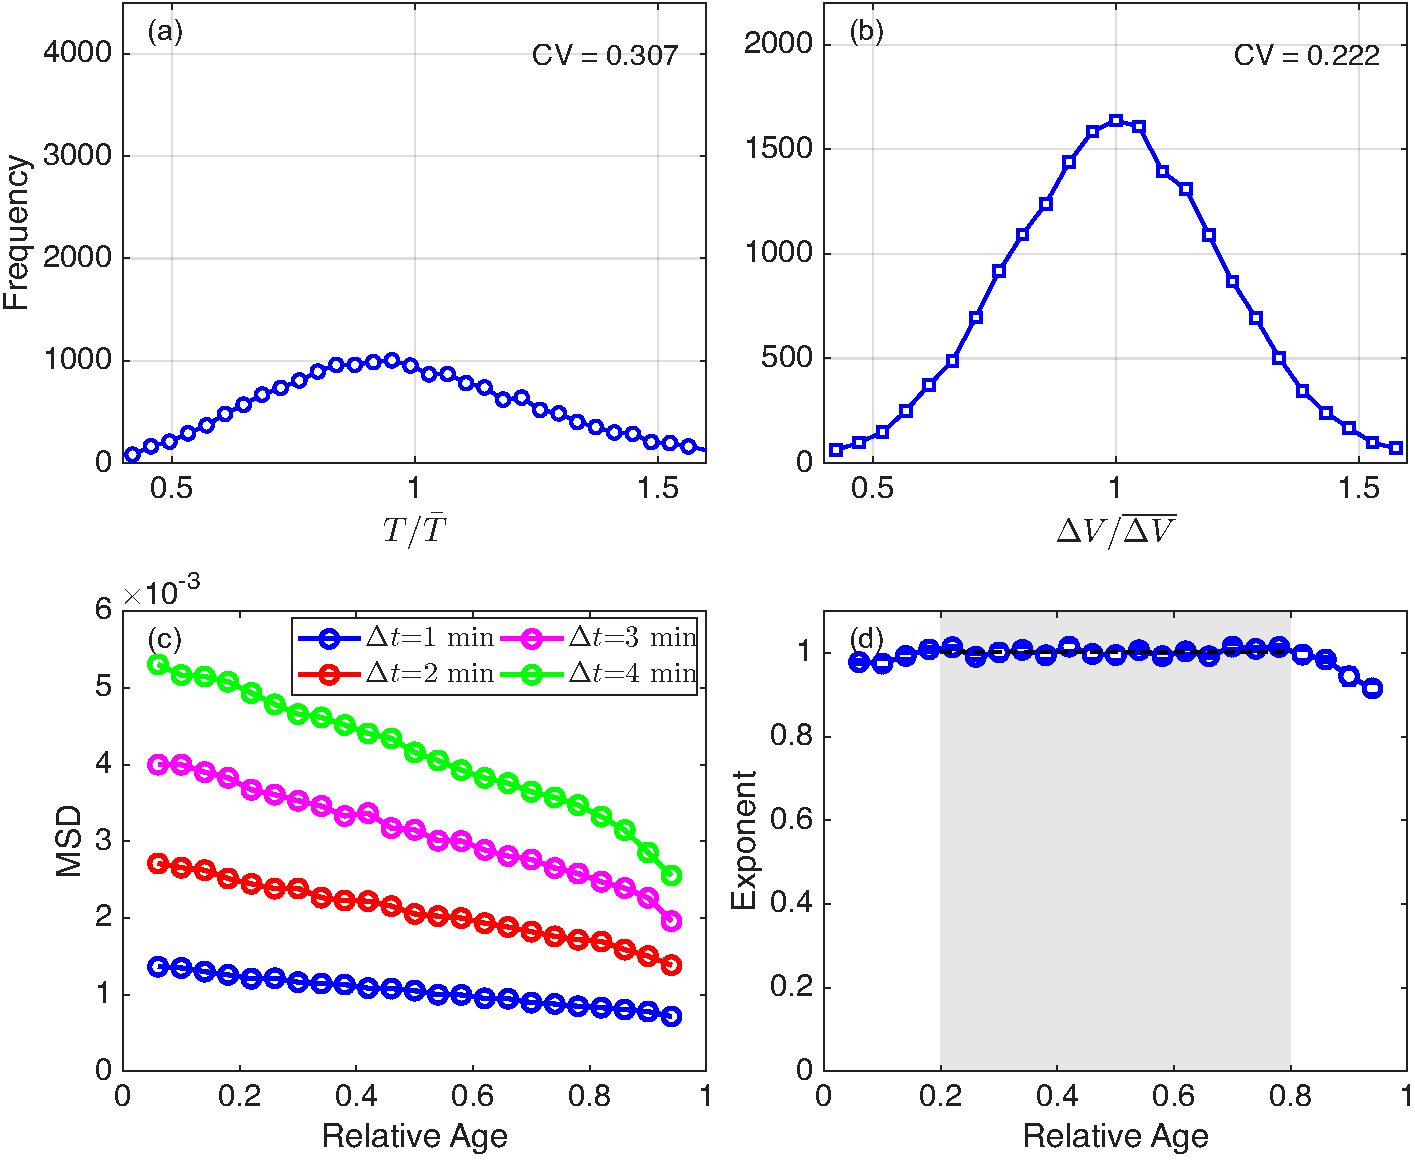
\includegraphics[width=0.8\textwidth]{sqrtV.pdf}
	\caption{Simulation results of the null model driven by $1/\sqrt{V}$ white noise. (a-b) Distributions of the normalized cell doubling time $T/\overline{T}$ (a) and normalized added volume $\Delta V/\overline{\Delta V}$ (b). (c) MSD vs. relative age at different time intervals. Distinct from the experimental results [Fig.~2(d) in the main text], MSD shows a pronounced decrease as relative age increases, validating the physical rationale of the null model in which the noise magnitude is $x$-independent. (d) The diffusion exponent ($\alpha$) calculated from the simulation data remains constant at 1 as a function of the relative age. Our conclusions for the null model remain the same, including the broad doubling-time distribution and the normal diffusion of random cell growth, even if we assume a noise magnitude that is $x$-dependent.}
	\label{fig:sqrtV}
\end{figure}


\end{document}